% !TEX TS-program = pdflatex
% !TEX encoding = UTF-8 Unicode

% This is a simple template for a LaTeX document using the "article" class.
% See "book", "report", "letter" for other types of document.

\documentclass[10pt]{article} % use larger type; default would be 10pt

\usepackage[utf8]{inputenc} % set input encoding (not needed with XeLaTeX)
\usepackage{titlesec}
\usepackage{amsmath}
%%% Examples of Article customizations
% These packages are optional, depending whether you want the features they provide.
% See the LaTeX Companion or other references for full information.

%%% PAGE DIMENSIONS
\usepackage{geometry} % to change the page dimensions
\geometry{a4paper} % or letterpaper (US) or a5paper or....
\geometry{margin=0.5in} % for example, change the margins to 2 inches all round
% \geometry{landscape} % set up the page for landscape
%   read geometry.pdf for detailed page layout information

\usepackage{graphicx} % support the \includegraphics command and options

% \usepackage[parfill]{parskip} % Activate to begin paragraphs with an empty line rather than an indent

%%% PACKAGES
\titleformat{\subsection}[runin]% runin puts it in the same paragraph
        {\normalfont\bfseries}% formatting commands to apply to the whole heading
        {\thesubsection}% the label and number
        {0.5em}% space between label/number and subsection title
        {}% formatting commands applied just to subsection title
        [.]
\usepackage{booktabs} % for much better looking tables
\usepackage{array} % for better arrays (eg matrices) in maths
\usepackage{paralist} % very flexible & customisable lists (eg. enumerate/itemize, etc.)
\usepackage{verbatim} % adds environment for commenting out blocks of text & for better verbatim
\usepackage{subfig} % make it possible to include more than one captioned figure/table in a single float
% These packages are all incorporated in the memoir class to one degree or another...

%%% HEADERS & FOOTERS
\usepackage{fancyhdr} % This should be set AFTER setting up the page geometry
\pagestyle{fancy} % options: empty , plain , fancy
\renewcommand{\headrulewidth}{0pt} % customise the layout...
\lhead{}\chead{}\rhead{}
\lfoot{}\cfoot{\thepage}\rfoot{}

%%% SECTION TITLE APPEARANCE
\usepackage{sectsty}
\allsectionsfont{\sffamily\mdseries\upshape} % (See the fntguide.pdf for font help)
% (This matches ConTeXt defaults)

%%% ToC (table of contents) APPEARANCE
\usepackage[nottoc,notlof,notlot]{tocbibind} % Put the bibliography in the ToC
\usepackage[titles,subfigure]{tocloft} % Alter the style of the Table of Contents
\renewcommand{\cftsecfont}{\rmfamily\mdseries\upshape}
\renewcommand{\cftsecpagefont}{\rmfamily\mdseries\upshape} % No bold!

%%% END Article customizations

%%% The "real" document content comes below...
\makeatletter
\renewcommand\subsection{\@startsection{subsection}{2}{\z@}%
                                     {-3.25ex\@plus -1ex \@minus -.2ex}%
                                     {-1.5ex \@plus .2ex}%
                                     {\normalfont\large\bfseries}}
\renewcommand\subsubsection{\@startsection{subsubsection}{3}{\z@}%
                                     {-3.25ex\@plus -1ex \@minus -.2ex}%
                                     {-1.5ex \@plus .2ex}%
                                     {\normalfont\normalsize\bfseries}}
\makeatother
\title{STU33009: Statistical Methods for Computer Science - Final Assignment
}
\author{Efeosa Eguavoen 17324649}
%\date{} % Activate to display a given date or no date (if empty),
         % otherwise the current date is printed 
\begin{document}
\maketitle
\newpage
\section{Question 1}
\subsection{(a)}
Given the exam can have any combination of 3 topics, and there's no replacement of topics, we can use the \(nCk\) formula to calculate how many combinations of topics we can have as we can also ignore the order. Using \(nCk = C(n,k)= \frac{n!} {(n-k)! × k!} \) and using  10 for \(n\) and 3 for \(k\) we get \(10C3 = C(10,3)= \frac{10!} {(10-3)! × 3!} =  120\) 
\subsection{(b)}
We can get the probability of none of the subjects we studied coming up by removing however many subjects we studied from the pool of selectable subjects, i.e if we studied 4 subjects, we'd have \(10-4\) subjects to choose 3 from. Based off this, we can derive the formula: \(\frac{(10-n)C3}{10C3}\) for \(n < 8\) as if we study 8 or more subjects one of them will definitely appear on the paper. This gives us the probability none of the subjects we studied come up.
\subsection{(c)}
The probability of failure is when less than 2 of the subjects we studied coming up or in other words, the probability of 0 subjects coming up or the probability of only one subject coming up. We already derived the probability of none of our subjects coming up in (c) so we only need to alter the numberof subjects that appear from our pool of subjects to get the probability of one subject coming up. We also need to multiply the number of subjects that don't come up in the pool. Doing this, we arrive at the formula: \(\frac{(nC1) * ((10-n)C2)}{10C3}\). Adding the probabilty of getting 0 subjects come up and one subject come up we get:
\[\frac{(10-n)C3}{10C3} + \frac{(nC1) * ((10-n)C2)}{10C3} \] for \(n < 8 \). For 8 subjects we only have to use \(\frac{(nC1) * ((10-n)C2)}{10C3}\). If you study 9 or 10 subjects you can't fail.
\subsection{(d)}
For 4 questions, it's largely the same we just have to adjust how many we can pick. \[\frac{(10-n)C4}{10C4} + \frac{(nC1) * ((10-n)C3)}{10C4} \] for \(n < 7 \). For 7 it's just \(\frac{(nC1) * ((10-n)C3)}{10C4}\). 8 and up you can't fail as too many subjects come up.
\begin{figure}[h]
    \centering
    \subfloat[4 questions]{{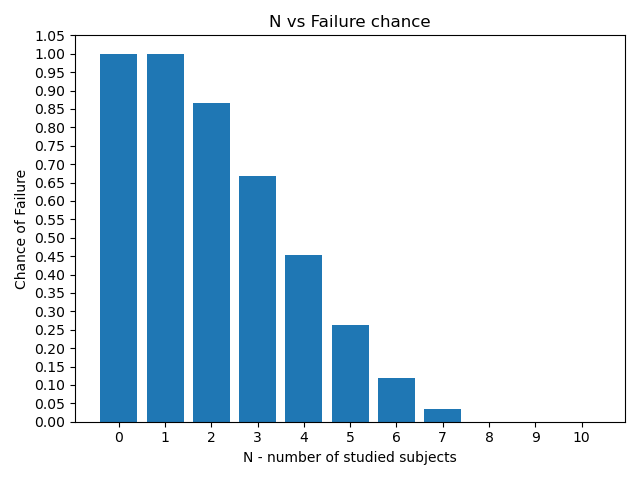
\includegraphics[width=6cm]{myplot.png} }}
    \qquad
    \subfloat[3 v 4]{{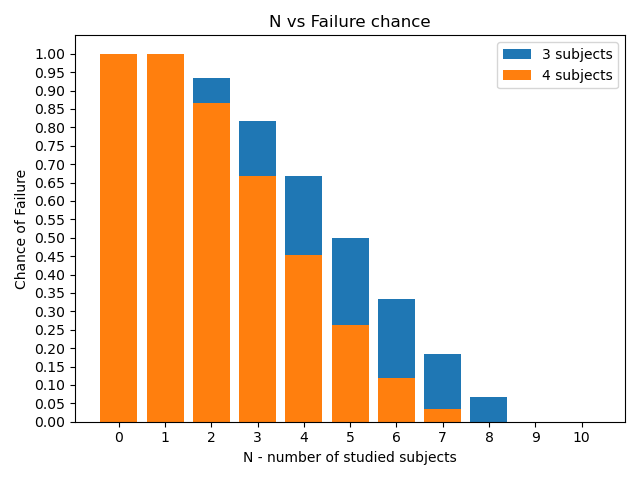
\includegraphics[width=6cm]{3v4.png} }}
    \label{fig:example}
\end{figure}
\newline
\textbf{Discussion} In regards to part c, when there's 4 questions on the paper, it makes it easier for a student to pass than when there's 3 questions. This effect seems to scale up as more questions are studied as when only 2 questions are studied the effect is about 5\% but when 4 are studied the effect is around 20\%. Also the minimum amount of questions necessary to pass is reduced by one also down to 8 questions. 
\subsection{(e)}
Simulation pseudo-code:
\newline
userList = random n subjects from 10
\newline
testList = random 3 subjects from 10
\newline
tot = 0
\newline
for item in userList:
\newline
	\indent if item in testList: tot++
	\newline
	\indent if tot == 2: return 1
	\newline
return 0 
\newline
To pick subjects randomly without replacement, I used the command \newline numpy.random.choice([subjects],n,replacement=False).
\newline This command assumes subjects has a uniform distribution i.e each item in subjects is as likely as any other to come up, but probabilities can be specified. The function in the code showing this is stoch\_sim()
\subsection{(f)}
Extending out the simulation,I just put a for loop around the call to the stochastic simulation in the main function.
\begin{equation}
\begin{split}
E[X_i] = 1-(\frac{7C0 * 3C3}{10C3} + \frac{7C1 * 3C2}{10C3}) \\
E[X_i] = 1- .18333333\\
E[X_i] = \frac{49}{60}\\
Var(X_i) = \frac{1}{N}\sum_{i =1}^N(X_i-E[X_i])^2 = \\
CLT(95\% Confidence) = \mu \pm 2\sigma \\
For N = 1000 \\
Var(X_i) = \frac{1}{1000}\sum_{i =1}^N(X_i-E[X_i])^2
Var(X_i) = .146977777778, Mean = .821\\
Confidence = [.821 - 2(\sqrt{.14697777778/1000}),.821+2(\sqrt{.14697777778/1000})] =[0.797,.845]\\
For N = 10000 \\
Var(X_i) = \frac{1}{10000}\sum_{i =1}^N(X_i-E[X_i])^2
Var(X_i) = .149321, Mean = .8173\\
Confidence = [.8173 - 2(\sqrt{.149321/10000}),.821+2(\sqrt{.149321/10000})] =[.8096,.8250]\\
\end{split}
\end{equation}
\subsection{(g)}
\begin{figure}[h]
\centering
    \subfloat[Scatter vs 95\% Confidence]{{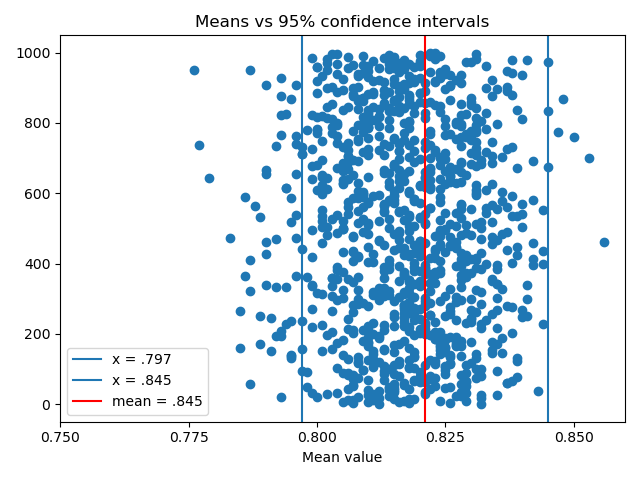
\includegraphics[width=8cm]{scatter1k.png} }}

    \label{fig:example}
\end{figure}
For N = 1000, I ran it 1000 times to generate 1000 points to see how well my confidence interval fit the data. From the plot above, we can see the around 95\% of all points fit within 2 standard deviations of the mean, with only a few outliers. I went with 1000 runs as I wanted to have a large enough value it would be very clear if my confidence interval is correct or not.
\begin{figure}[h]
\centering
    \subfloat[Scatter vs 95\% Confidence]{{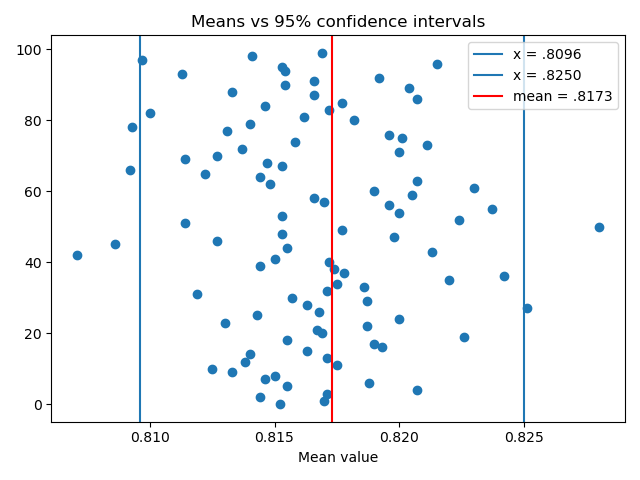
\includegraphics[width=8cm]{scatter1m.png} }}

    \label{fig:example}
\end{figure}
\newline
For N = 10,000 I ran it 100 times only as it's quite computationally expensive to run it 1000 times as 10,000 scores need to be calculated each time. From the plot, we can count only 5 points falling outside the 95\% confidence interval which is inline with what we'd expect. The accuracy is what we'd expect from this level of confidence. 
\subsection{(h)}
If the test becomes predicatble based on the previous years test, I came up with 2 possible strategies students can take:
\newline
A student could possibly choose n subjects from the ones that came up next year and then depending on how many more they wish to study, pick at random from the other subjects. i.e subjects that came up last get first preference then everything else.For when a subject is less likely, they pick from the main pool first then the pool of subjects that came up.
\newline
Another strategy is to leave the subjects in a pool and then weight the probabilities of the subjects based on when they came up. Then pick n at random.
\newline
Pseudocode:
\newline
pickedList = random(3 items from subjects list, picked according to their possible weighted probabilities)
\newline
testList  =  random(3 items from subject list, by new weighted probabilities from previous year)
\newline for item in pickedList:
\newline
	\indent if item in testList: tot++
	\newline
	\indent if tot == 2: return 1
	\newline
return 0 
\newline recalculate probabilites
\newline
Other function\newline
pList = [] (List of subjects that didn't come up last year)\newline
olist = []
for item in prevList:
\newline \indent if item not in prevList: add to pList \newline
\indent else: add to olist \newline
userList = random \newline
userList += random(n-3 from plist) \newline
The rest is the same as  normal stochastic simulation.\newline
recalculate probabilites based on test results\newline
The functions in the code to calculate these results can be found at probalter() which calculates new probabilities,stoch\_alter() and stoch\_alter2() that are the 2 different methods I mentioned above.\newline
\textbf{Results}
\begin{figure}[h]
    \centering
    \subfloat[Method 1]{{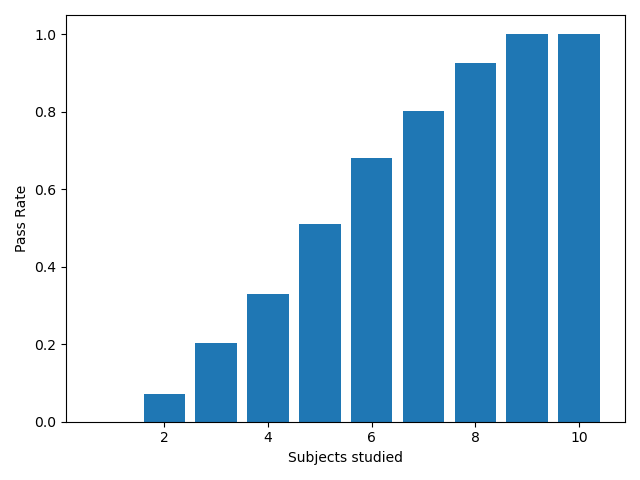
\includegraphics[width=5cm]{p1.png} }}
    \qquad
    \subfloat[Method 2]{{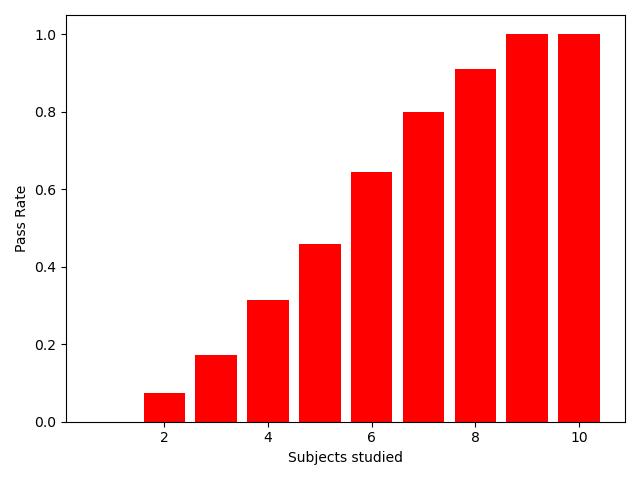
\includegraphics[width=5cm]{p4.png} }}
    \label{fig:example}
\end{figure}
From my simulation, as the exam became more predictable, the students that used the pooling method seemed to pass more often on average than students who did tried to use the probabilities and poll randomly. This is probably due to the fact that questions that came up last year were more likely to repeat or not repeat so by changing the pool to seperate them, they increased their likelihood of succes, especially when they were studying less subjects. This effect seemed to become more and more negligible as more subjects are studied. But overall, making the exam more predicatble and students attempting to predict topics seemed to increase the overall pass rate.
\begin{figure}[h]
    \centering
    \subfloat[Method 1v2]{{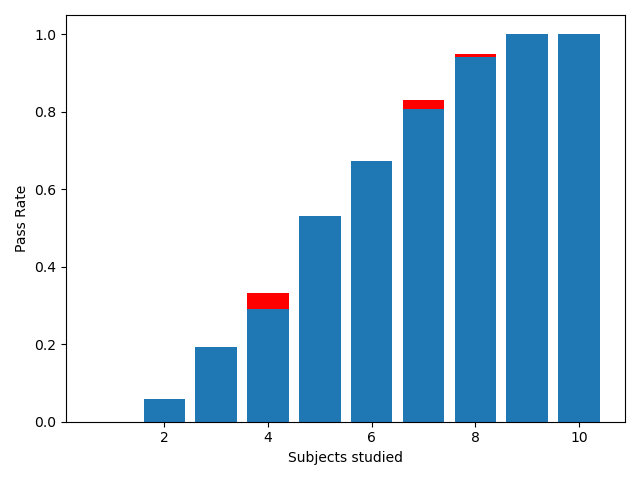
\includegraphics[width=5cm]{p5.png} }}
    \label{fig:example}
\end{figure}
\newline
\newline
As for when the exam was still conducted normally i.e all subjects had equal chance of coming up, students that used the pooling method fared worse overall with many more failing over the number of tests. By attempting to predict the questions, they were weighting the questions wrongly and essentially eliminating questions that had just as much chance to appear, and as a result failing more often. The students that left everything as one pool did better as not picking at random using some sort of weighted probability seemed to level things out for them rather than picking with priority.
\section{Question 2} id:0.548:0.5-0.314:2-0.614:2-0
\subsection{(a)}
I split it into different questions, then counted up the amount of times each number ocurred and put it over the amout of data points given. As for binning, I left it in bins of 5 as that's how the data we were given came and it enabled me to represent the data as we were given. To plot the pmf's, I used matplotlib.bar() with the data we were given. The functions in the code that correspond to this are datagrab(),pmfmake().
\begin{figure}[h]
    \centering
    \subfloat[Question 1]{{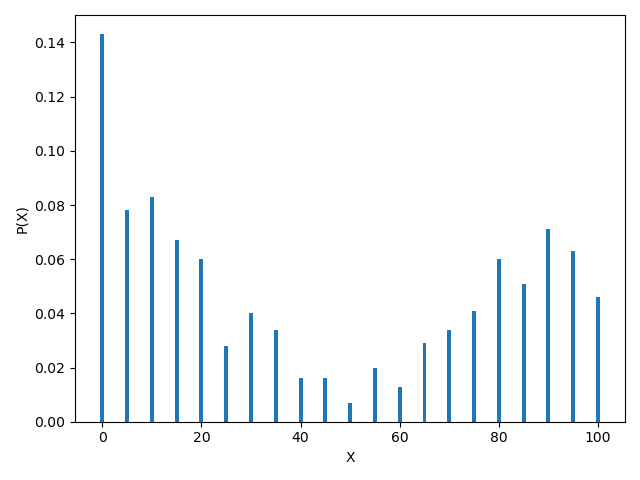
\includegraphics[width=4cm]{pmf1.png} }}
    \qquad
    \subfloat[Question 2]{{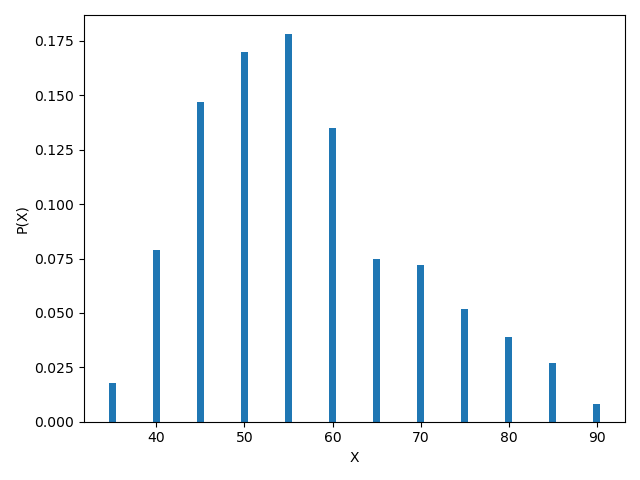
\includegraphics[width=4cm]{pmf2.png} }}
     \qquad
    \subfloat[Question 3]{{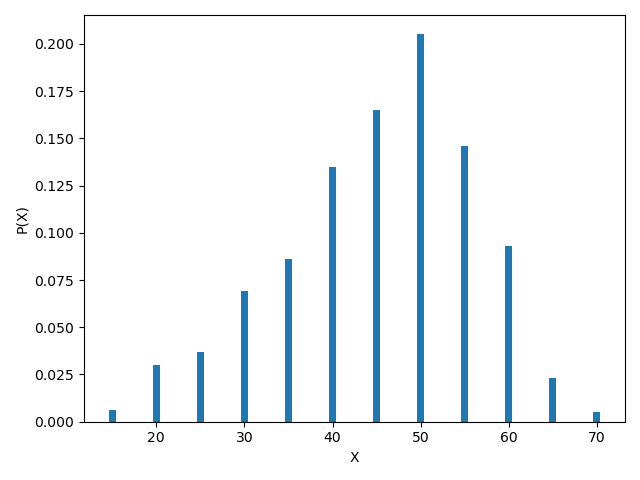
\includegraphics[width=4cm]{pmf3.png} }}
    \label{fig:example}
\end{figure}
From the PMF's it seems Question 1 or Question 3 are the most difficult question based off the spread of the results. While Question 3 seems gaussian, looking at the range of scores, the scores do not go any higher than 70\% while in Question 1, the scores are concentrated at both ends of the spectrum, which could indicate the question may not be that difficult but is dependant on the students preparation.Question 2 is the easiest of the 3 with all the results sitting above 35\% and a large majority being 50+.Using a PMF to evaluate difficulty can be useful as a very basic measure of difficulty as we can see all the data on it's own but having no real comparison of difficulty or cross referencing keeps it rather basic as a metric of difficulty. We can't see a real distibution of the scores and confidence intervals and such, leaving it rather basic.

\subsection{(b)}
Results:
\newline

I used bins of size 5 as the dataset was incremental in sizes of 5. Binning is useful as we can group students by grade and compare and contrast them across. I decided not to use a larger bin size as it might make me lose some accuracy which wouldn't be favourable as my results would be altered by some amount. As for calculating the means and the variances, once the results were binned, I just summed the bins and divided by the amount in each bin. For the variance, I subtracted the mean from each result, summed the results and divided by the amount. This can be seen in the meVar() function.
\subsection{(c)} For this question, I calculated the means of each of the questions by using the bins from the previous question, then I got the variance for each respective bin to get the standard deviation. I used 65\% for each point as 95\% was unnecessary and made it harder to analyse the graphs properly. I then used matplotlib.errorbar() to create the error bar plots, using the standard deviations and the means. The ErrorBar() plots the bars while the rest of it was done in line at the bottom of the code.
\begin{figure}[h]
    \centering
    \subfloat[Q2 conditioned on Q1]{{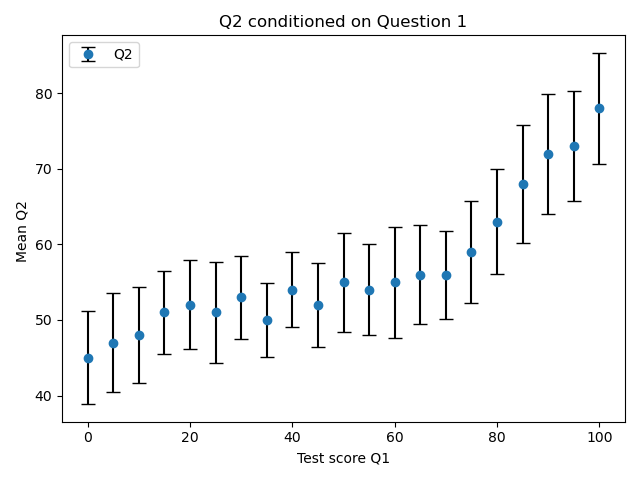
\includegraphics[width=5cm]{error1.png} }}
    \qquad
    \subfloat[Q3 conditioned on Q1]{{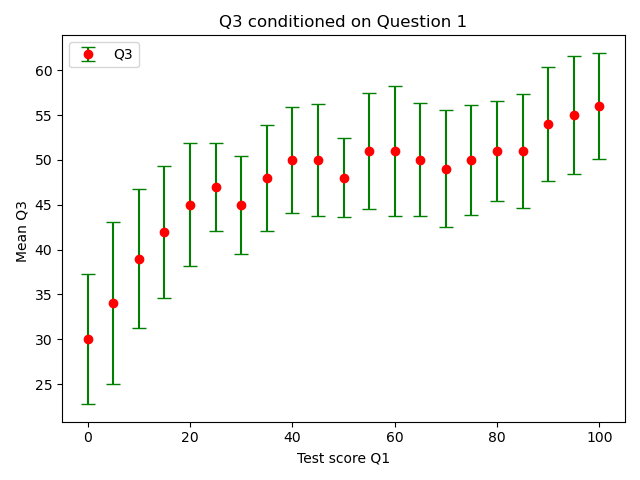
\includegraphics[width=5cm]{error2.png} }}
     \qquad
    \subfloat[Q3 v Q2 conditioned on Q1]{{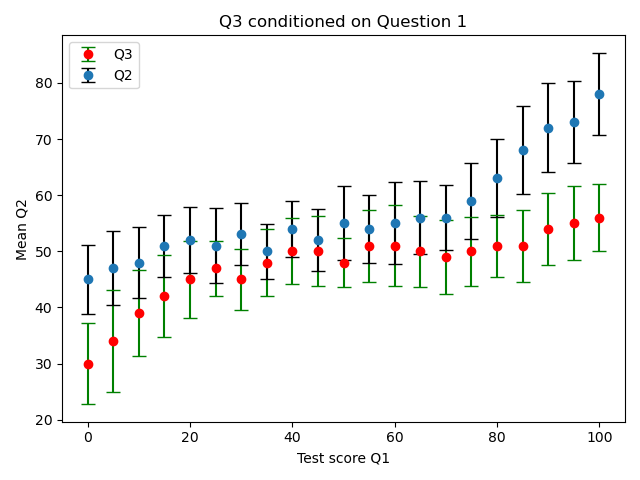
\includegraphics[width=5cm]{error3.png} }}
    \label{fig:example}
\end{figure}
\newline
\textbf{Discussion} From the error bar charts, we can clearly see question 2 to be the easiest of the questions. The mean of Q3 for students with the same mark in Q1 doesn't fall within 1 standard deviation in most cases other than in the center. We can also see that students of average ability seem to get roughly the same score in each question the how close the means are and are all within 1 standard deviation of each other. Overall we can see Q3 to be the most difficult to do well in but Q1 still seems to be the most difficult to pass as a large number of students are getting between 0 and 30, which we can verify due to the large standard deviations at that end of the graph. 
\subsection{(d)}
X = input Feature(Q1 results) , Y = Output(Qx result)
\newline m = training data(The dataset). We can split the data into training and testing so we can test how good our model is after we've made it.
\newline Assuming the data has a linear fit, we can then use \(J(\theta_0,\theta_1)=\frac{1}{m}\sum_{i=1}^{m}(h_\theta(x^i)-y^(i))^2\) or the least squares method to minimise the cost function. From here we can use Gradient Descent to find \(\theta\) that minimised \(J(\theta)\). Finally we're left with \(y = h_\theta(x) = \theta_0 +\theta_1x\) (assuming it's linear). We can then use the test data and look at the residuals to construct a confidence interval for our model.
\newline
The assumption that the mean is a linear function of the features isn't appropriate here in my opinion as while it's possible to fit a linear line through the data, it would be an underfit of the data. The data presents more of a sigmoid function than linear. To better fit the data, we could define a new feature that is a function of the curve the data suggest i.e \(\frac{1}{1+e^{-x}}\) with some tweaks could fit the data a lot better than a linear function. We do need to be careful we don't overfit the data although by selecting a feature that goes through all the data points. From here we can use linear regression as normal to fit the model which I think would better, more accurate predictions. 
\newline
I don't think the type of randomness associated with linear regression is appropriate here as we have bounds on our inputs as inputs can only be between 0-100 and so can the outputs.While the input in this range is random, it's not wholly random like in normal linear regression.
\newpage
\section{Code}
I split the code into multiple functions as it's easier to reference from the report.
\begin{verbatim}
import random
import numpy as np
import pandas as pd
import matplotlib.pyplot as plt
import math
def stoch_sim(n: int):
    subjectList = [1,2,3,4,5,6,7,8,9,10]
    pickedList = list(np.random.choice(subjectList,n,False))
    testList = list(np.random.choice(subjectList,3,False))
    onTest = 0
    state = 0
    for i in pickedList:
        if i in testList:
            onTest = onTest+1
        if onTest==2:
            state = 1
            return state
    return state
def dataGrab():
    q1 = []
    q2 = []
    q3 = []
    datafile = open("final2020.txt","r")
    for i in datafile:
        vals = i.split(" ")
        q1.append(int(vals[0]))
        q2.append(int(vals[1]))
        q3.append(int(vals[2]))
    df = pd.DataFrame.from_records([q1, q2, q3])
    df = df.transpose()
    data1 = pd.DataFrame(df[0].value_counts())
    data1.columns = ["Counts"]
    data1["Prob"] = data1["Counts"] / 1000
    data2 = pd.DataFrame(df[1].value_counts())
    data2.columns = ["Counts"]
    data2["Prob"] = data2["Counts"] / 1000
    data3 = pd.DataFrame(df[2].value_counts())
    data3.columns = ["Counts"]
    data3["Prob"] = data3["Counts"] / 1000
    print(data1,"\n \n",data2,"\n \n",data3)
    return ((q1,data1),(q2,data2),(q3,data3))
def pmf_make(data):
    pmf = plt.bar(data.index.values, data["Prob"])
    plt.xlabel("X")
    plt.ylabel("P(X)")
    plt.show()
def stoch_alter(n,probs,testList):
    subjectList = [1, 2, 3, 4, 5, 6, 7, 8, 9, 10]
    pickedList = list(np.random.choice(subjectList, n, False,probs))
    onTest = 0
    state = 0
    for i in pickedList:
        if i in testList:
            onTest = onTest + 1
        if onTest == 2:
            state = 1
            return state,testList
    return state, testList
def stoch_alter2(n,prevTest,probs,testList):
    subjectList = [1, 2, 3, 4, 5, 6, 7, 8, 9, 10]
    alterList = []
    for i in subjectList:
        if i not in prevTest:
            alterList.append(i)
    alterWay = []
    if n <= 3:
        alterWay = list(np.random.choice(prevTest, n, False))
    else:
        alterWay = list(np.random.choice(prevTest, 3, False))
        alterWay =  alterWay + (list(np.random.choice(alterList, n - 3, False)))
    onTest = 0
    state = 0
    for i in alterWay:
        if i in testList:
            onTest = onTest + 1
        if onTest == 2:
            state = 1
            return state,testList
    return state, testList
def main():
    results = [0,0,0,0,0,0,0,0,0,0]
    specRes = []
    means = []
    for i in range(100):
        specRes = []
        for s in range(10000):
            val = stoch_sim(7)
            specRes.append(val)
        if(len(specRes) != 0):
            mean = sum(specRes) / len(specRes)
            means.append(mean)
    print(len(means))
    plt.scatter(means,np.arange(0,100,1))
    plt.axvline(x=.8096,label = "x = .8096")
    plt.axvline(x=.8250, label = "x = .8250")
    plt.axvline(x=0.8173, color="r",label = "mean = .8173")
    plt.xlabel("Mean value")
    plt.title("Means vs 95\% confidence intervals")
    plt.legend()
    plt.show()
    for i in range(len(specRes)):
        specRes[i] = (specRes[i]-(49/60))**2
    total = sum(specRes)
    print(total/10000)
    print(mean)
def probalter(prob,s,prevTest):
    total = 0
    for i in prevTest:
        prev = prob[i-1]
        prob[i-1] = prob[i-1] * s
        total = total + (prob[i-1] - prev)
    dec = total/7
    for i in range(len(prob)):
        if i+1 not in prevTest:
            prob[i] = prob[i] - dec
    print(sum(prob))
    return prob
def meVar(dicter):
    means = []
    vars = []
    for item in dicter.items():
        mean = sum(item[1])/len(item[1])
        var = 0
        for items in item[1]:
            cur = (items-mean)**2
            var = cur + var
        var = var/len(item[1])
        means.append((item[0],mean))
        vars.append(var)
    return means,vars
def errorBars(means,vars,m2,v2):
    plt.clf()
    ms = [i[0] for i in means]
    nms = [int(i[1]) for i in means]
    ms2 = [i[0] for i in m2]
    nms2 = [int(i[1]) for i in m2]
    plt.errorbar(ms2,nms2,v2,fmt='ro',ecolor='green',capsize=5,barsabove=False,label="Q3")
    plt.errorbar(ms, nms, vars, fmt='o', ecolor='black', capsize=5, barsabove=False,label="Q2")
    plt.xlabel("Test score Q1")
    plt.ylabel("Mean Q2")
    plt.title("Q2 v Q3 conditioned on Question 1")
    plt.legend()
    plt.show()
def fails():
    vals = []
    v2 = []
    for i in range(11):
        val = (math.comb(10-i,4)/math.comb(10,4)) + ((i*(math.comb(10-i,3)))/math.comb(10,4))
        vals.append((i,val))
    for i in range(11):
        val = (math.comb(10 - i, 3) / math.comb(10, 3)) + ((i * (math.comb(10 - i, 2))) / math.comb(10, 3))
        v2.append((i, val))
    print(vals)
    print(v2)
    plt.bar([i[0] for i in v2], [i[1] for i in v2], ecolor="green",label="3 subjects")
    plt.bar([i[0] for i in vals],[i[1] for i in vals],ecolor="black",label="4 subjects")
    plt.xlabel("N - number of studied subjects")
    plt.ylabel("Chance of Failure")
    plt.title("N vs Failure chance")
    plt.xticks(np.arange(0,11,1))
    plt.yticks(np.arange(0.0,1.05,.05))
    plt.legend()
    plt.show()
if __name__ == '__main__':
    init_probs = [.1, .1, .1, .1, .1, .1, .1, .1, .1, .1]
    q1,q2,q3 = dataGrab()
    bin2 = {}
    bin3 = {}
    for i in range(len(q1[0])):
        if q1[0][i] in bin2:
            bin2[q1[0][i]] = bin2[q1[0][i]] + [q2[0][i]]
            bin3[q1[0][i]] = bin3[q1[0][i]] + [q3[0][i]]
        else:
            bin2[q1[0][i]] = [q2[0][i]]
            bin3[q1[0][i]] = [q3[0][i]]
    means,vars = meVar(bin2)
    print(means)
    m2,var2 = meVar(bin3)
    vars = list(map(lambda x: (math.sqrt(x)),vars))
    var2 = list(map(lambda x: (math.sqrt(x)),var2))
\end{verbatim}
\end{document}
